\subsection{Segregation system}

\subsubsection{Check data balancing}

\begin{figure}[H]
\centering
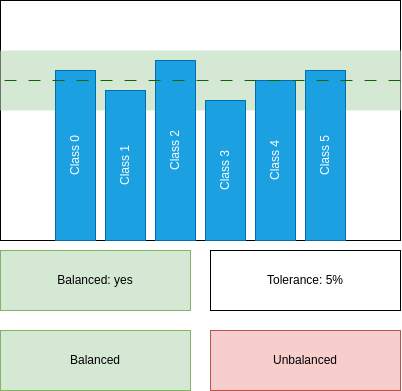
\includegraphics[width=0.8\textwidth]{figures/check_data_balancing.png}
\caption{"Check data balancing" mock-up form}
\end{figure}

\begin{table}[H]
\centering
\begin{tabular}{|l|c|c|c|c|}
\hline
\textbf{Step} & \textbf{O} & \textbf{CL} & \textbf{S} & \textbf{SC} \\
\hline
\textbf{1} \textbf{ACTOR} opens "Check data balancing" form. & & & & \\
\hline
\textbf{2} \textbf{SYSTEM} shows the report. & & & & \\
\hline
\textbf{3} \textbf{SYSTEM} shows a hint whether the data is balanced or not. & & & & \\
\hline
\textbf{4} \textbf{ACTOR} checks threshold in the UI. & & & & \\
\hline
\textbf{5} \textbf{FOR} each column in the report: & & & & \\
\hline
\textbf{5.1} \textbf{IF} the column is not within the displayed threshold. & & & & \\
\hline
\textbf{5.1.1} \textbf{THEN} the data is not balanced. & & & & \\
\hline
\textbf{6.1} \textbf{IF} the data is balanced. & & & & \\
\hline
\textbf{6.1.1} \textbf{ACTOR} clicks "Balanced" button. & & & & \\
\hline
\textbf{6.2} \textbf{ELSE} & & & & \\
\hline
\textbf{6.2.1} \textbf{ACTOR} clicks "Unbalanced" button. & & & & \\
\hline
\textbf{7} \textbf{SYSTEM} shows a confirmation dialog. & & & & \\
\hline
\textbf{8} \textbf{ACTOR} closes the form. & & & & \\
\hline
\multicolumn{4}{|r|}{Human task cost} & \\
\hline
\end{tabular}
\caption{Detailed use case for "Check data balancing" task}
\label{table:check_data_balancing}
\end{table}

\subsubsection{Check input coverage}

\begin{figure}[H]
\centering
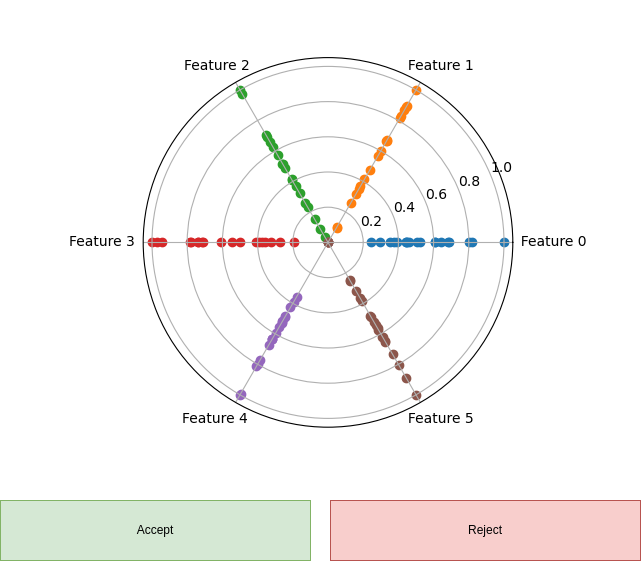
\includegraphics[width=0.8\textwidth]{figures/check_input_coverage.png}
\caption{"Check input coverage" mock-up form}
\end{figure}

\begin{table}[H]
\centering
\begin{tabular}{|l|c|c|}
\hline
\textbf{Step} & \textbf{Cost calculation} & \textbf{SC} \\
\hline
\textbf{1} \textbf{ACTOR} opens "Check input coverage" form. & & \\
\hline
\textbf{2} \textbf{SYSTEM} shows a radar scatter plot of the input distribution. & & \\
\hline
\textbf{3} \textbf{FOR} each radius in the radar scatter plot: & & \\
\hline
\textbf{3.1} \textbf{IF} the distribution is not uniform as expected. & & \\
\hline
\textbf{3.1.1} \textbf{THEN} the input coverage is not satisfied. & & \\
\hline
\textbf{4.1} \textbf{IF} the input coverage is satisfied. & & \\
\hline
\textbf{4.1.1} \textbf{ACTOR} clicks "Accept" button. & & \\
\hline
\textbf{4.2} \textbf{ELSE} & & \\
\hline
\textbf{4.2.1} \textbf{ACTOR} clicks "Reject" button. & & \\
\hline
\textbf{5} \textbf{SYSTEM} shows a confirmation dialog. & & \\
\hline
\textbf{6} \textbf{ACTOR} closes the form. & & \\
\hline
\multicolumn{2}{|r|}{Human task cost} & \\
\hline
\end{tabular}
\caption{Detailed use case for "Check input coverage" task}
\label{table:check_input_coverage}
\end{table}



\subsection{Development system}

\subsubsection{Set iteration number}

\begin{figure}[H]
\centering
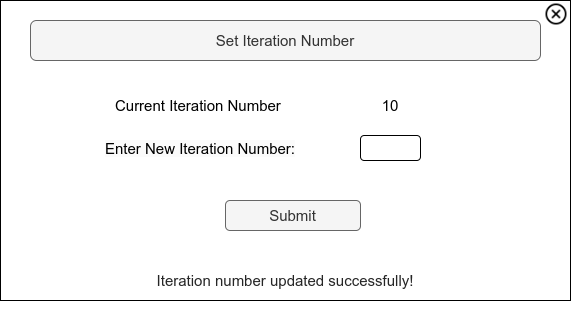
\includegraphics[width=0.8\textwidth]{figures/set_iteration_number.png}
\caption{"Set iteration number" mock-up form}
\end{figure}

\begin{table}[H]
\centering
\begin{tabular}{|l|c|c|}
\hline
\textbf{Step} & \textbf{Cost calculation} & \textbf{SC} \\
\hline
\textbf{1} \textbf{ACTOR} opens "Set Iteration Number" form. & & \\
\hline
\textbf{2} \textbf{SYSTEM} displays the current iteration number. & & \\
\hline
\textbf{3} \textbf{ACTOR} inputs the desired number of iterations. & & \\
\hline
\textbf{4} \textbf{ACTOR} clicks "Submit" button to confirm the iteration number. & & \\
\hline
\textbf{5} \textbf{SYSTEM} shows a confirmation dialog. & & \\
\hline
\textbf{6} \textbf{ACTOR} closes the form. & & \\
\hline
\end{tabular}
\caption{Detailed use case for "Set iteration number" task}
\label{table:set_iteration_number}
\end{table}